% Template for Cogsci submission with R Markdown

% Stuff changed from original Markdown PLOS Template
\documentclass[10pt, letterpaper]{article}

\usepackage{cogsci}
\usepackage{pslatex}
\usepackage{float}
\usepackage{caption}

% amsmath package, useful for mathematical formulas
\usepackage{amsmath}

% amssymb package, useful for mathematical symbols
\usepackage{amssymb}

% hyperref package, useful for hyperlinks
\usepackage{hyperref}

% graphicx package, useful for including eps and pdf graphics
% include graphics with the command \includegraphics
\usepackage{graphicx}

% Sweave(-like)
\usepackage{fancyvrb}
\DefineVerbatimEnvironment{Sinput}{Verbatim}{fontshape=sl}
\DefineVerbatimEnvironment{Soutput}{Verbatim}{}
\DefineVerbatimEnvironment{Scode}{Verbatim}{fontshape=sl}
\newenvironment{Schunk}{}{}
\DefineVerbatimEnvironment{Code}{Verbatim}{}
\DefineVerbatimEnvironment{CodeInput}{Verbatim}{fontshape=sl}
\DefineVerbatimEnvironment{CodeOutput}{Verbatim}{}
\newenvironment{CodeChunk}{}{}

% cite package, to clean up citations in the main text. Do not remove.
\usepackage{apacite}

% KM added 1/4/18 to allow control of blind submission


\usepackage{color}

% Use doublespacing - comment out for single spacing
%\usepackage{setspace}
%\doublespacing


% % Text layout
% \topmargin 0.0cm
% \oddsidemargin 0.5cm
% \evensidemargin 0.5cm
% \textwidth 16cm
% \textheight 21cm

\title{Peekbank: Exploring children's word recognition through an open,
large-scale repository for developmental eye-tracking data}

\usepackage[raggedright]{sidecap}

\author{{\large \bf Martin Zettersten (martincz@princeton.edu)} \\ Department of Psychology, South Dr \\ Princeton, NJ 08540 USA \AND {\large \bf Claire Bergey (cbergey@uchicago.edu)} \AND {\large \bf Naiti S. Bhatt (naitibhatt@gmail.com)}  \AND {\large \bf Veronica Boyce (vboyce@stanford.edu)} \AND {\large \bf Mika Braginsky (mikabr@mit.edu)} \AND {\large \bf Alexandra Carstensen (abcarstensen@stanford.edu)}  \AND {\large \bf Benny deMayo (bdemayo@princeton.edu)}  \AND {\large \bf George Kachergis (kachergis@stanford.edu)}  \AND {\large \bf Molly Lewis (mollyllewis@gmail.com)} \AND {\large \bf Bria Long (bria@stanford.edu)} \AND {\large \bf Kyle MacDonald (kylem412@gmail.com)} \AND {\large \bf Jessica Mankewitz (jmankewitz@stanford.edu)} \AND {\large \bf Stephan Meylan (smeylan@mit.edu)}  \AND {\large \bf Annissa N. Saleh (ans638@nyu.edu)} \AND {\large \bf Rose M. Schneider (roschnei@ucsd.edu)}  \AND {\large \bf Angeline Sin Mei Tsui (astsui@stanford.edu)}   \AND {\large \bf Sarp Uner (sarp.uner@duke.edu)}  \AND {\large \bf Tian Linger Xu (txu@iu.edu)}  \AND {\large \bf Daniel Yurovsky (yurovsky@stanford.edu)}  \AND {\large \bf Michael C. Frank (mcfrank@stanford.edu)}}


\begin{document}

\maketitle

\begin{abstract}
The ability to rapidly recognize words and link them to referents in
context is central to children's early language development. This
ability, often called word recognition in the developmental literature,
is typically studied in the looking-while-listening paradigm, which
measures infants' fixation of a target object (vs.~a distractor) after
hearing a target label. We present a large-scale, open database of
infant and toddler eye-tracking data from looking-while-listening tasks.
The goal of this effort is to address theoretical and methodological
challenges in measuring infant vocabulary development. We present two
analyses of the current database (N=1,233): (1) capturing age-related
changes in infants' word recognition while generalizing across
item-level variability and (2) assessing how a central methodological
decision -- selecting the time window of analysis -- impacts the
reliability of measurement. Future efforts will expand the scope of the
current database to advance our understanding of participant-level and
item-level variation in children's vocabulary development.

\textbf{Keywords:}
word recognition; eye-tracking; vocabulary development;
looking-while-listening
\end{abstract}

\hypertarget{introduction}{%
\section{Introduction}\label{introduction}}

Across their first years of life, children learn words in their native
tongues at a rapid pace (Frank, Braginsky, Yurovsky, \& Marchman, 2021).
A key part of the word learning process is children's ability to rapidly
process words and link them to relevant meanings - often referred to as
word recognition. Developing word recognition skills builds a foundation
for children's language development and is predictive of later
linguistic and general cognitive outcomes (Bleses, Makransky, Dale,
Højen, \& Ari, 2016; Marchman et al., 2018).

Word recognition is traditionally studied in the
``looking-while-listening'' paradigm (alternatively referred to as the
intermodal preferential looking procedure; Fernald, Zangl, Portillo, \&
Marchman, 2008; Hirsh-Pasek, Cauley, Golinkoff, \& Gordon, 1987). In
such studies, infants listen to a sentence prompting a specific referent
(e.g., \emph{Look at the dog!}) while viewing two images on the screen
(e.g., an image of a dog - the target image - and an image of a duck -
the distractor image). Infants' word recognition is measured in terms of
how quickly and accurately they fixate the correct target image after
hearing its label. Studies using this design have contributed to our
understanding of a wide range of questions in language development,
including infants' early noun knowledge, phonological representations of
words, prediction during language processing, and individual differences
in language development (Bergelson \& Swingley, 2012; Golinkoff, Ma,
Song, \& Hirsh-Pasek, 2013; Lew-Williams \& Fernald, 2007; Marchman et
al., 2018; Swingley \& Aslin, 2000).

While the looking-while-listening paradigm has been highly fruitful in
advancing understanding of early word knowledge, fundamental questions
remain both about the trajectory of children's word recognition ability
and the nature of the method itself. One central question is how to
measure developmental change in word recognition. Age-related changes
and individual differences in speed of word recognition are thought to
support children's subsequent language learning (e.g., Marchman \&
Fernald, 2008). However, measuring increases in speed and accuracy of
word recognition faces the challenge of distinguishing developmental
changes in word recognition skill from changes in knowledge of specific
words. This problem is particularly thorny in child development, since
the number of items that can be tested within a single session is
limited and items must be selected in an age-appropriate manner (Peter
et al., 2019). Measuring developmental change therefore requires
large-scale datasets with a range of items, in order to generalize
age-related changes across words.

A second question relates to evaluating methodological best practices.
In particular, many fundamental analytic decisions vary substantially
across studies, and different decisions may lead to different inferences
about children's word recognition. For example, researchers vary in how
they select time windows for analysis, transform the dependent measure
of target fixations, and model the time course of word recognition
(Csibra, Hernik, Mascaro, Tatone, \& Lengyel, 2016; Fernald et al.,
2008; Huang \& Snedeker, 2020). This problem is made more complex by the
fact that many of these decisions depend on a variety of design-related
and participant-related factors (e.g., infant age). Establishing best
practices therefore requires a large database of infant word recognition
studies varying across such factors, in order to test the potential
consequences of methodological decisions on study results.

What these two questions share is that they are difficult to answer at
the scale of a single study. To address this challenge, we introduce
\emph{Peekbank}, a flexible and reproducible interface to an open
database of developmental eye-tracking studies. The Peekbank project (a)
collects a large set of eye-tracking datasets on children's word
recognition, (b) introduces a data format and processing tools for
standardizing eye-tracking data across data sources, and (c) provides an
API for accessing and analyzing the database. In the current paper, we
give an overview of the key components of the project and some initial
demonstrations of its utility in advancing theoretical and
methodological insights. We report two analyses using the database and
associated tools (N=1,233): (1) a growth-curve analysis modeling
age-related changes in infants' word recognition while generalizing
across item-level variability and (2) a multiverse-style analysis of how
a central methodological decision -- selecting the time window of
analysis -- impacts inter-item reliability.

\hypertarget{methods}{%
\section{Methods}\label{methods}}

\hypertarget{database-framework}{%
\subsection{Database Framework}\label{database-framework}}

\begin{CodeChunk}
\begin{figure}[tb]

{\centering \includegraphics{figs/fig_framework_overview-1} 

}

\caption[Overview of the Peekbank data ecosystem]{Overview of the Peekbank data ecosystem. Peekbank tools are highlighted in green. *custom R packages.}\label{fig:fig_framework_overview}
\end{figure}
\end{CodeChunk}

The Peekbank data framework consists of three libraries that take in raw
experimental datasets, populate a relational database, and provide an
API interface (Fig. \ref{fig:fig_framework_overview}). The
\texttt{peekds} library (for the R language) helps researchers convert
and validate existing datasets to use the relational format used by the
database. The \texttt{peekbank} library (Python) creates a database with
the relational schema and populates it with the standardized datasets
produced by \texttt{peekds}. The database is implemented in MySQL, an
industry standard relational database, which may be accessed by a
variety of programming languages over the internet. The
\texttt{peekbankr} library (R) provides an application programming
interface, or API, that provides high-level abstractions to help
researchers run common analysis tasks on the database.

\hypertarget{data-format-and-processing}{%
\subsection{Data Format and
Processing}\label{data-format-and-processing}}

One of the main challenges in compiling a large-scale eye-tracking
dataset is the lack of a shared re-usable data format across individual
experiments. Researcher conventions for structuring data vary, as do the
technical specifications of different devices, rendering the task of
integrating datasets from different labs and data sources difficult. We
developed a common, \texttt{tidy} format for the eye-tracking data in
Peekbank to ease the process of conducting cross-dataset analyses
(Wickham et al., 2019). The schema of the database is sufficiently
general to handle heterogeneous datasets, including both manually coded
and automated eye-tracking data.

During data import, raw eye-tracking datasets are processed to conform
to the Peekbank data schema. The centerpiece of the schema is the
aoi\_timepoints table (Fig. \ref{fig:fig_framework_overview}), which
records whether participants looked to the target or the distractor
stimulus at each timepoint of a given trial. Additional tables track
information about data sources, participant characteristics, trial
characteristics, stimuli, and raw eye-tracking data. In addition to
unifying the data format, we conduct several additional pre-processing
steps to facilitate analyses across datasets, including resampling
observations to a common sampling rate (40 Hz) and normalizing time
relative to the onset of the target label.

\hypertarget{current-data-sources}{%
\subsection{Current Data Sources}\label{current-data-sources}}

\begin{table}[H]
\centering
\begingroup\fontsize{9pt}{10pt}\selectfont
\begin{tabular}{lrrl}
  \hline
Dataset Name & N & Mean Age & Method \\ 
  \hline
canine & 36 & 23.8 & manual coding \\ 
  coartic & 29 & 20.8 & eye-tracking \\ 
  cowpig & 45 & 20.5 & manual coding \\ 
  ft\_pt & 69 & 17.1 & manual coding \\ 
  reflook\_socword & 435 & 33.6 & eye-tracking \\ 
  reflook\_v4 & 347 & 37.2 & eye-tracking \\ 
  salientme & 44 & 40.1 & manual coding \\ 
  switchingCues & 60 & 44.3 & manual coding \\ 
  tablet & 110 & 33.8 & eye-tracking \\ 
  tseltal & 23 & 31.3 & manual coding \\ 
  yoursmy & 35 & 14.5 & eye-tracking \\ 
   \hline
\end{tabular}
\endgroup
\caption{Overview over the datasets in the current database.} 
\end{table}

The database currently includes 11 looking-while-listening datasets
comprising N=1233 total participants (Table 1). Most datasets (10 out of
11 total) consist of data from monolingual native English speakers. They
span a wide age spectrum with participants ranging from 8 to 84 months
of age, and are balanced in terms of gender (48\% female). The datasets
vary across a number of dimensions related to design and methodology,
and include studies using manually coded video recordings and automated
eye-tracking methods (e.g., Tobii, EyeLink) to measure children's gaze
behavior. Most studies focused on testing familiar items, but the
database also includes studies with novel pseudowords. All data (and
accompanying references) are openly available on the Open Science
Framework
(\url{https://osf.io/pr6wu/?view_only=07a3887eb7a24643bdc1b2612f2729de}).

\sidecaptionvpos{figure}{c}
\begin{SCfigure*}[0.2] 
\includegraphics[width=14cm,height=8.4cm]{../figures/peekbank_item_vis.png}
\caption{Item-level variability in proportion target looking within each dataset (chance=0.5). Time is centered on the onset of the target label (vertical line). Colored lines represent specific target labels. Black lines represent smoothed average fits based on a general additive model using cubic splines.}
\label{fig:peekbank_item_vis}
\end{SCfigure*}

\hypertarget{results}{%
\section{Results}\label{results}}

\hypertarget{general-descriptives-and-item-variability}{%
\subsection{General descriptives and item
variability}\label{general-descriptives-and-item-variability}}

\begin{table}[H]
\centering
\begingroup\fontsize{9pt}{10pt}\selectfont
\begin{tabular}{lrrl}
  \hline
Dataset Name & Unique Items & Prop. Target & 95\% CI \\ 
  \hline
canine & 16 & 0.64 & [0.61, 0.67] \\ 
  coartic & 10 & 0.70 & [0.67, 0.73] \\ 
  cowpig & 12 & 0.60 & [0.58, 0.63] \\ 
  ft\_pt & 8 & 0.64 & [0.63, 0.66] \\ 
  reflook\_socword & 6 & 0.61 & [0.6, 0.63] \\ 
  reflook\_v4 & 10 & 0.63 & [0.61, 0.64] \\ 
  salientme & 16 & 0.73 & [0.71, 0.75] \\ 
  switchingCues & 40 & 0.77 & [0.75, 0.79] \\ 
  tablet & 24 & 0.53 & [0.51, 0.56] \\ 
  tseltal & 30 & 0.59 & [0.54, 0.63] \\ 
  yoursmy & 87 & 0.60 & [0.55, 0.64] \\ 
   \hline
\end{tabular}
\endgroup
\caption{Average proportion target looking in each dataset.} 
\end{table}

In general, participants demonstrated robust, above-chance word
recognition in each dataset (with chance being 0.5). Table 2 shows the
average proportion of target looking within a standard critical window
of 300 - 2000ms after the onset of the label for each dataset (Swingley
\& Aslin, 2000). The number of unique target labels and their associated
accuracy vary widely across datasets (Figure
\ref{fig:peekbank_item_vis}). Proportion target looking was generally
higher for familiar words (M = 67.5\%, 95\% CI = {[}66.6\%, 68.5\%{]})
than for novel words learned during the experiment (M = 55.1\%, 95\% CI
= {[}53.8\%, 56.3\%{]}).

\hypertarget{predicting-age-related-changes-while-generalizing-across-items}{%
\subsection{Predicting Age-Related Changes While Generalizing Across
Items}\label{predicting-age-related-changes-while-generalizing-across-items}}

\sidecaptionvpos{figure}{c}
\begin{SCfigure*}[0.2] 
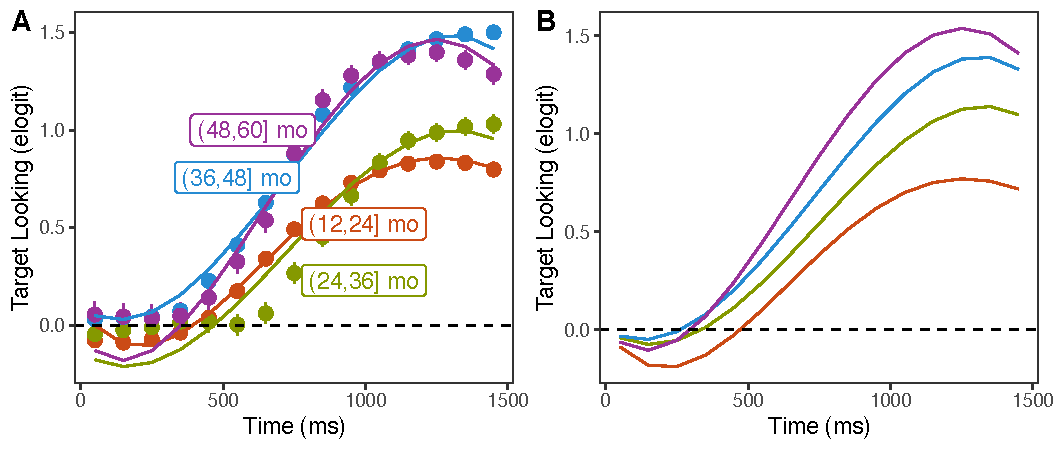
\includegraphics[width=14cm,height=6cm]{../figures/age_gca.png}
\caption{Growth curve models of proportion target looking during the critical target window at each age range (in months). (A) Mean empirical word recognition fit. (B) Population-level estimates.}
\label{fig:age_gca}
\end{SCfigure*}

Developmental changes in word recognition have been a central issue
since early investigations of eye-tracking techniques (Fernald, Pinto,
Swingley, Weinberg, \& McRoberts, 1998). Children's speed and accuracy
of word recognition increases across early childhood, yet measuring
these increases presents an item selection puzzle for researchers: Words
that are appropriate for an 18-month-old will be too easy for a
three-year-old; those that are appropriate for a three-year-old will be
difficult for the 18-month-old. Failure to choose appropriate test items
can even lead to spurious conclusions about development (Peter et al.,
2019).

This issue is familiar in psychometrics: test developers interested in
measuring across a wide range of a particular latent ability must choose
items appropriate for different abilities. One solution is to use data
from a bank of questions that have been taken by test-takers of a range
of abilities, and then use item-response theory models to create
different test versions appropriate for different ability ranges
(Embretson \& Reise, 2000). Such tests can then be used to extract
estimates of developmental change that are independent of individual
tests and their particular items.

Peekbank provides the appropriate large-scale database for estimating
these item-independent developmental changes and designing
age-appropriate tests in the future. Here we show a proof of concept by
providing an estimate of the item-independent growth of word recognition
accuracy across development. We take advantage of the equivalence
between item response theory and linear mixed effects models (LMMs; De
Boeck et al., 2011), using LMMs to model the trajectory of word
recognition across age. We follow the approach of Mirman (2014) and use
growth curve LMMs to predict the time course of recognition.
Specifically, we predicted children's proportion of target looking
during an early window of time (0 - 1500ms, chosen to avoid modeling
declines in looking later in the trial), using an empirical logit
transform on the proportion of target looking to allow the use of linear
(rather than logistic) regression models. Our predictors were time after
word onset and age, and we additionally included polynomial functions of
time (up to fourth order) and quadratic effects of age, as well as their
interactions. We subtracted all intercepts to force fits to start at a
baseline of 0 (chance performance) at time zero. As a random effect
structure, we included by-item, by-subject, and by-dataset random
intercepts; though a larger random effect structure could be justified
by the data, the size of the dataset precluded fitting these. The random
effect structure allows us to model word recognition while generalizing
across items and participants.

Figure \ref{fig:age_gca} depicts the results of this analysis. Panel A
shows the mean empirical word recognition curves for four age groups,
along with fitted model performance. Although model fits are acceptable,
developmental change appears irregular - for example, 12--24 month-olds
show slightly earlier recognition than 24--36 month-olds. This pattern
is likely an artifact of averaging across datasets with substantially
different items and structures. Panel B shows model predictions for the
population level of each random effect -- our best estimates of the
latent ability structure. Here we see continuous increases in both speed
(point at which the curve rises) and accuracy (asymptote of the curve)
across ages, though this developmental trend decelerates (consistent
with other work on reaction time development; Frank, Lewis, \&
MacDonald, 2016; Kail, 1991). This proof of concept suggests that
Peekbank can be used to model developmental change over multiple years,
overcoming the limitations of individual datasets.

\hypertarget{time-window-selection}{%
\subsection{Time Window Selection}\label{time-window-selection}}

\begin{SCfigure*}[0.3] 
\includegraphics[width=14cm,height=8.75cm]{../figures/interitem_cors_window_analysis.png}
\caption{Participants' average inter-item correlation for proportion of looking time to familiar targets, as a function of window start time and end time, with each facet showing a different age group. More positive (red) correlations are more desirable, and blue/white represent start/end time combinations that researchers should avoid.}
\label{fig:time_window}
\end{SCfigure*}

In our second analysis, we addressed a common analytic decision facing
researchers: how to summarize time course data into a single measure of
accuracy. Taking a similar approach to that of Peelle \& Van Engen
(2020), we conducted a multiverse-style analysis considering possible
time windows researchers might select (Steegen, Tuerlinckx, Gelman, \&
Vanpaemel, 2016). Our multiverse analysis focuses on the reliability of
participants' response to familiar words by measuring the subject-level
inter-item correlation (IIC) for proportion of looking at familiar
targets. The time windows selected by researchers varies substantially
in the literature, with some studies analyzing shorter time windows
between 300 ms and 1800-2000 ms post-target onset (Fernald et al., 2008;
Swingley \& Aslin, 2000), and others using longer time windows extending
to approximately 3000-4000ms (especially with younger infants; e.g.,
Bergelson \& Swingley, 2012). We thus examined a broad range of window
start times ranging from 300 ms pre-target onset to 1500 ms post-target
onset and window end times ranging from 0 ms to 4000 ms post-target
onset. For each combination of window start time and end time with a
minimum window duration of 50 ms, we calculated participants' average
inter-item correlation for proportion of looking at familiar targets
(mean IIC). Since observations were unevenly distributed across the age
range, and because children likely show a varying response to familiar
items as they age (often motivating different window choices), we split
our data into four age bins (12-24, 24-36, 36-48, and 48-60 months).
While it is an open question what space of possible windows will yield
the greatest reliability, we expect to see low reliability (i.e.~0) in
windows that start before target onset and in windows that end within
300 ms post-target onset, before participants are able to execute a
response.

Results from this multiverse analysis are shown in Figure
\ref{fig:time_window}, where each colored pixel represents the mean IIC
for proportion of looking to familiar targets for a specific combination
of window start and end time. The analysis shows that IIC is positive
(red) under a wide range of sensible window choices. IIC is relatively
low however, especially for the youngest age group, suggesting that
individual items carry only limited shared signal regarding children's
underlying ability. It may be the case that even averaging many such
trials does not yield highly reliable measures of individual
differences, although some multi-trial paradigms are exceptions to this
generalization (Fernald et al., 2008).

Intriguingly, however, late end times and long overall window lengths
show the greatest reliability. Shorter windows (e.g., 300-2000ms, as we
used above) likely maximize absolute recognition performance by fitting
the peak of the recognition curve, but simultaneously lower reliability
by failing to include all relevant data. Especially for older children,
the maximal IICs were found with windows that started between 500 and
1000ms and ended between 3000 and 4000ms, windows usually reserved for
younger children. This finding is sensible from a psychometric
perspective -- averaging more timepoints (even if some contain limited
signal) increases reliability and reduces variation. Thus, researchers
interested in better measurement of individual variation or condition
differences should consider using longer windows by default.

\hypertarget{discussion}{%
\section{Discussion}\label{discussion}}

Theoretical progress in understanding child development requires rich
datasets, but collecting child data is expensive, difficult, and
time-intensive. Recent years have seen a growing effort to build open
source tools and pool research efforts to meet the challenge of building
a cumulative developmental science (Bergmann et al., 2018; The
ManyBabies Consortium, 2020). The Peekbank project expands on these
efforts by building an infrastructure for aggregating eye-tracking data
across studies, with a specific focus on the looking-while-listening
paradigm. This paper presents an illustration of some of the key
theoretical and methodological questions that can be addressed using
Peekbank: generalizing across item-level variability in children's word
recognition and providing data-driven guidance on methodological
choices.

Our first analysis shows that Peekbank can be used to model
item-independent changes in the speed and accuracy of word recognition
across development. Children showed age-related increases in the speed
of word recognition across one to five years of age, extending past
foundational work (e.g., Fernald et al., 1998) by showing that these
word processing gains generalize across items and are not only
attributable word-specific gains in processing speed. The second
analysis demonstrates how Peekbank can be used to make principled,
data-driven analytic decisions, specifically the choice of time windows
for analyzing developmental eye-tracking data. In
looking-while-listening studies, researchers often choose a relatively
short time window of roughly 300-1800 or 2000 ms (Fernald et al., 2008),
with the justification that eye movements occurring after this window
may no longer reflect fixations related to the target label (Swingley \&
Aslin, 2000). Our results recommend that researchers consider increasing
the size of the time window for analyzing target fixations (at least for
familiar words) to maximize the consistent signal present in children's
target fixations.

There are a number of critical limitations surrounding the current scope
of the database. A key priority in future work will be to expand the
size of the database. With 11 datasets currently available in the
dataset, idiosyncrasies of particular designs and condition
manipulations still have substantial influence on modeling results.
Expanding the set of distinct datasets will allow us to increase the
number of observations per item across datasets, allowing for more
robust generalizations regarding participant- and item-level
variability. The current database is also limited by the relatively
homogeneous background of its participants, both with respect to
language (almost entirely monolingual native English speakers) and
cultural background (all but one dataset comes from WEIRD environments;
Muthukrishna et al., 2020). Increasing the diversity of participant
backgrounds and languages will increase the scope of the generalizations
we can form about child word recognition.

Finally, while the current database is mainly focused on studies of word
recognition, the tools and infrastructure developed in the project can
in principle be expanded to accommodate any eye-tracking paradigm used
with infants and toddlers, opening up new avenues for insights into
infant development. Infant looking has been at the core of many of the
key advances in our understanding of infant cognition. Aggregating large
datasets of infant looking behavior in a single, openly-accessible
format promises to bring a fuller picture of infant cognitive
development into view.

\hypertarget{acknowledgements}{%
\section{Acknowledgements}\label{acknowledgements}}

We would like to thank the labs and researchers that have made their
data publicly available in the database.

\hypertarget{references}{%
\section{References}\label{references}}

\setlength{\parindent}{-0.1in} 
\setlength{\leftskip}{0.125in}

\noindent

\hypertarget{refs}{}
\leavevmode\hypertarget{ref-Bergelson2012a}{}%
Bergelson, E., \& Swingley, D. (2012). At 6-9 months, human infants know
the meanings of many common nouns. \emph{PNAS}, \emph{109}(9),
3253--3258.

\leavevmode\hypertarget{ref-Bergmann2018}{}%
Bergmann, C., Tsuji, S., Piccinini, P. E., Lewis, M. L., Braginsky, M.,
Frank, M. C., \& Cristia, A. (2018). Promoting replicability in
developmental research through meta-analyses: Insights from language
acquisition research. \emph{Child Development}, \emph{89}(6),
1996--2009.

\leavevmode\hypertarget{ref-Bleses2016}{}%
Bleses, D., Makransky, G., Dale, P. S., Højen, A., \& Ari, B. A. (2016).
Early productive vocabulary predicts academic achievement 10 years
later. \emph{Applied Psycholinguistics}, \emph{37}(6), 1461--1476.

\leavevmode\hypertarget{ref-Csibra2016}{}%
Csibra, G., Hernik, M., Mascaro, O., Tatone, D., \& Lengyel, M. (2016).
Statistical treatment of looking-time data. \emph{Developmental
Psychology}, \emph{52}(4), 521--536.

\leavevmode\hypertarget{ref-de-boeck2011}{}%
De Boeck, P., Bakker, M., Zwitser, R., Nivard, M., Hofman, A.,
Tuerlinckx, F., \ldots{} others. (2011). The estimation of item response
models with the lmer function from the lme4 package in r. \emph{Journal
of Statistical Software}, \emph{39}(12), 1--28.

\leavevmode\hypertarget{ref-embretson2000}{}%
Embretson, S. E., \& Reise, S. P. (2000). \emph{Item response theory for
psychologists}. Mahwah, NJ: Lawrence Erlbaum Associates.

\leavevmode\hypertarget{ref-fernald1998}{}%
Fernald, A., Pinto, J. P., Swingley, D., Weinberg, A., \& McRoberts, G.
W. (1998). Rapid gains in speed of verbal processing by infants in the
2nd year. \emph{Psychological Science}, \emph{9}(3), 228--231.

\leavevmode\hypertarget{ref-Fernald2008}{}%
Fernald, A., Zangl, R., Portillo, A. L., \& Marchman, V. A. (2008).
Looking while listening: Using eye movements to monitor spoken language
comprehension by infants and young children. In I. A. Sekerina, E. M.
Fernandez, \& H. Clahsen (Eds.), \emph{Developmental psycholinguistics:
On-line methods in children's language processing} (pp. 97--135).
Amsterdam: John Benjamins.

\leavevmode\hypertarget{ref-frank2021}{}%
Frank, M. C., Braginsky, M., Yurovsky, D., \& Marchman, V. A. (2021).
\emph{Variability and Consistency in Early Language Learning: The
Wordbank Project}. Cambridge, MA: MIT Press.

\leavevmode\hypertarget{ref-frank2016b}{}%
Frank, M. C., Lewis, M., \& MacDonald, K. (2016). A performance model
for early word learning. In \emph{Proceedings of the 38th annual
conference of the cognitive science society} (pp. 2610--2614). Austin,
TX: Cognitive Science Society.

\leavevmode\hypertarget{ref-Golinkoff2013}{}%
Golinkoff, R. M., Ma, W., Song, L., \& Hirsh-Pasek, K. (2013).
Twenty-five years using the intermodal preferential looking paradigm to
study language acquisition: What have we learned? \emph{Perspectives on
Psychological Science}, \emph{8}(3), 316--339.

\leavevmode\hypertarget{ref-Hirsh-Pasek1987}{}%
Hirsh-Pasek, K., Cauley, K. M., Golinkoff, R. M., \& Gordon, L. (1987).
The eyes have it: Lexical and syntactic comprehension in a new paradigm.
\emph{Journal of Child Language}, \emph{14}(1), 23--45.

\leavevmode\hypertarget{ref-Huang2020}{}%
Huang, Y., \& Snedeker, J. (2020). Evidence from the visual world
paradigm raises questions about unaccusativity and growth curve
analyses. \emph{Cognition}, \emph{200}, 104251.

\leavevmode\hypertarget{ref-kail1991}{}%
Kail, R. (1991). Developmental change in speed of processing during
childhood and adolescence. \emph{Psychological Bulletin}, \emph{109}(3),
490.

\leavevmode\hypertarget{ref-Lew-Williams2007}{}%
Lew-Williams, C., \& Fernald, A. (2007). Young children learning Spanish
make rapid use of grammatical gender in spoken word recognition.
\emph{Psychological Science}, \emph{18}(3), 193--198.

\leavevmode\hypertarget{ref-Marchman2008}{}%
Marchman, V. A., \& Fernald, A. (2008). Speed of word recognition and
vocabulary knowledge in infancy predict cognitive and language outcomes
in later childhood. \emph{Developmental Science}, \emph{11}(3), F9--16.

\leavevmode\hypertarget{ref-Marchman2018}{}%
Marchman, V. A., Loi, E. C., Adams, K. A., Ashland, M., Fernald, A., \&
Feldman, H. M. (2018). Speed of language comprehension at 18 months old
predicts school-relevant outcomes at 54 months old in children born
preterm. \emph{Journal of Developmental \& Behavioral Pediatrics},
\emph{39}(3), 246--253.

\leavevmode\hypertarget{ref-Mirman2014}{}%
Mirman, D. (2014). \emph{Growth curve analysis and visualization using
R}. Boca Raton, FL: CRC Press.

\leavevmode\hypertarget{ref-Muthukrishna2020}{}%
Muthukrishna, M., Bell, A. V., Henrich, J., Curtin, C. M., Gedranovich,
A., McInerney, J., \& Thue, B. (2020). Beyond Western, Educated,
Industrial, Rich, and Democratic (WEIRD) Psychology: Measuring and
Mapping Scales of Cultural and Psychological Distance.
\emph{Psychological Science}, \emph{31}(6), 678--701.

\leavevmode\hypertarget{ref-Peelle2020}{}%
Peelle, J. E., \& Van Engen, K. J. (2020). Time stand still: Effects of
temporal window selection on eye tracking analysis. \emph{PsyArXiv}.
\url{http://doi.org/https://doi.org/10.31234/osf.io/pc3da}

\leavevmode\hypertarget{ref-peter2019}{}%
Peter, M. S., Durrant, S., Jessop, A., Bidgood, A., Pine, J. M., \&
Rowland, C. F. (2019). Does speed of processing or vocabulary size
predict later language growth in toddlers? \emph{Cognitive Psychology},
\emph{115}, 101238.

\leavevmode\hypertarget{ref-steegenEtAl2016}{}%
Steegen, S., Tuerlinckx, F., Gelman, A., \& Vanpaemel, W. (2016).
Increasing transparency through a multiverse analysis.
\emph{Perspectives on Psychological Science}, \emph{11}(5), 702--712.

\leavevmode\hypertarget{ref-Swingley2000}{}%
Swingley, D., \& Aslin, R. N. (2000). Spoken word recognition and
lexical representation in very young children. \emph{Cognition},
\emph{76}(2), 147--66.

\leavevmode\hypertarget{ref-TheManyBabiesConsortium2020}{}%
The ManyBabies Consortium. (2020). Quantifying sources of variability in
infancy research using the infant-directed speech preference.
\emph{Advances in Methods and Practices in Psychological Science},
\emph{3}(1), 24--52.

\leavevmode\hypertarget{ref-Wickham2019}{}%
Wickham, H., Averick, M., Bryan, J., Chang, W., McGowan, L. D.,
François, R., \ldots{} Yutani, H. (2019). Welcome to the tidyverse.
\emph{Journal of Open Source Software}, \emph{4}(43), 1686.

\bibliographystyle{apacite}


\end{document}
